\documentclass{beamer}
  \usepackage[english]{babel}
  \usepackage[utf8]{inputenc}
  \usepackage{times}
  \usepackage{amsmath,amsthm, amssymb, latexsym,ragged2e}
  \boldmath
  
  \usetheme{Poster}
  \usepackage[orientation=portrait,size=a0,scale=1.4]{beamerposter}


  \title[Beamer Poster]{Application de la Morphogénèse de Réseaux Biologiques à la Conception Optimale d'Infrastructures de Transport}
  \author[<juste.raimbault,jorge.gonzalez-suitt>@polytechnique.edu]{J. Raimbault$^{1,2}$ et J.Gonzalez$^{2}$}
  \institute[]
  {$^1$ UMR CNRS 8504 - Géographie-Cités, $^2$ Ecole Polytechnique\vspace{1cm}}
  \date{\today}
  
  \logo{
  \hfill
  
\includegraphics[height=8cm,width=0.32\columnwidth]{figures/logo}
  
\includegraphics[height=8cm,width=0.32\columnwidth]{figures/geocite}
  
\includegraphics[height=8cm,width=0.32\columnwidth]{figures/logoX}
  \hfill\hfill
  }


  %%%%%%%%%%%%%%%%%%%%%%%%%%%%%%%%%%%%%%%%%%%%%%%%%%%%%%%%%%%%%%%%%%%%%%%%%%%%%%%%%5
  \begin{document}
  \begin{frame}{} 
  
    \vfill
    \begin{columns}[t]
      \begin{column}{.49\textwidth}
      
      
        \begin{block}{Introduction}
        \vspace{-1cm}
        \begin{columns}[t]
        \begin{column}{.95\textwidth}
          \begin{itemize}         
          \item \begin{justify}Conception des infrastructures de transport généralement \emph{top-down} (approche type modèles d'interaction transport-usage du sol~\cite{wegener2004land}).
          \end{justify}
          \bigskip
          \item \begin{justify}
          Récente introduction des méthodes de \emph{bio-mimétisme} pour le design et le management des systèmes technico-sociaux complexes~\cite{doursat2012morphogenetic}.
          \end{justify}
          \bigskip
          \item Application efficace aux infrastructures de transports par optimisation multi-objectif (ex. coût, robustesse) émergente~\cite{bebber2007biological}.
          \bigskip
          \item Dans notre cas, application d'un modèle de morphogénèse de \emph{slime mould} au design optimal de systèmes de transport.
          \end{itemize}
          \end{column}
          \end{columns}
        \end{block}
        
         \begin{block}{Modèle}
        %\vspace{-1cm}
        \begin{columns}[t]
        \begin{column}{.95\textwidth}
        \vspace{-2cm}
        \begin{justify}
          Modèle proposé dans~\cite{TeroAl10} : principe \emph{d'exploration puis renforcement} pour une moisissure à la recherche de ressources.
          
          \bigskip
          
          Etude de l'aspect renforcement : réseau initial homogène de tubes $ij$, longueur $L_{ij}$, diamètre variable $D_{ij}$, traversés par un flux de fluide $Q_{ij}$. Sommets $i$ à la pression $p_i$. Un nombre de noeuds $N$ sont à desservir, parmi eux aléatoirement à chaque étape l'un est source $p_{i_+}=I_0$ et l'autre puits $p_{i_-}=-I_0$
          
          
          \bigskip
          \textit{Itération du modèle :}
          \begin{enumerate}
          \item Détermination des flux par lois de Kirchoff (analogie électrostatique, résolution d'un système fermé) : loi d'Ohm
          \begin{equation}
Q_{ij}=\frac{D_{ij}}{L_{ij}}\cdot(p_{i}-p_{j})
\end{equation}
et conservation des flux
\begin{equation}
\sum_{j\rightarrow i}Q_{ij} = 0 , \sum_{j\rightarrow i_\pm}Q_{i_{\pm}j} = \pm I_0
\end{equation}



\item Evolution du diamètres de tubes ($\gamma$ paramètre de renforcement)
\begin{equation}
\frac{dD_{ij}}{dt}=\frac{\left|Q_{ij}\right|^{\gamma}}{1+\left|Q_{ij}\right|^{\gamma}}-D_{ij}
\end{equation}
          \end{enumerate}

\bigskip

Extraction du réseau final après convergence selon un paramètre de seuil de diamètre (distributions finales généralement bimodales).

\bigskip 

\textit{Modèle multi-échelle :} Dynamique des diamètres supposées constantes pendant l'itération pour obtenir les flux. 

\bigskip 

\textit{Implémentation en NetLogo ouverte~\cite{impl}}
\end{justify}
          \end{column}
          \end{columns}
        \end{block}
        
        
        \begin{block}{Indicateurs}
       \vspace{-2cm}
        \begin{columns}[t]
        \begin{column}{.95\textwidth}
        \begin{justify}
          Comportement du modèle évalué au travers d'indicateurs de performance pour le réseau généré $(V_f,E_f)$, qui peuvent être vu comme des objectifs contradictoires :
          \bigskip
          \begin{itemize}
          \item Coût de construction $c=\sum_{ij\in E_f}D_{ij}(t_f)$
          \bigskip
          \item \begin{justify}Performance moyenne~\cite{banos2012towards}
          \[
          v=\frac{1}{|V_f|^2}\sum_{i,j\in V_f}\frac{d_{i\rightarrow j}}{||\vec{i}-\vec{j}||}
          \]
          \end{justify}
          \bigskip
          \item Robustesse (indice \textit{Network Trip Robustness}~\cite{sullivan2010identifying})
          \end{itemize}

          \end{justify}
          \end{column}
          \end{columns}
        \end{block}
        
        
        \begin{block}{Analyse de Sensibilité}
       \vspace{-1cm}
        \begin{columns}[t]
        \begin{column}{.47\textwidth}
                    
          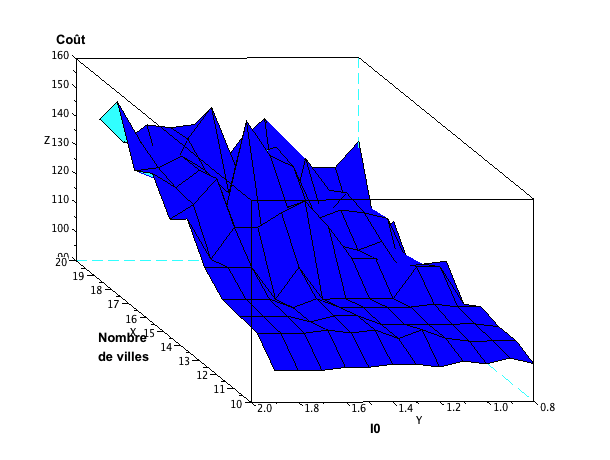
\includegraphics[width=0.5\columnwidth,height=8cm]{figures/graphe_cout}
          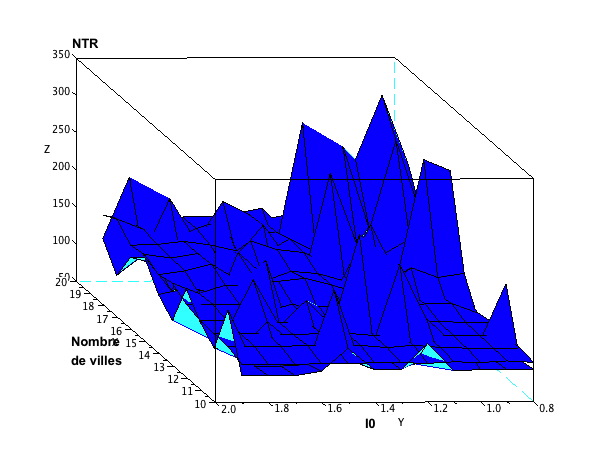
\includegraphics[width=0.5\columnwidth,height=8cm]{figures/graphe_NTR}\\
          \bigskip
          \textit{Sensibilité des indicateurs aux paramètres $(N,I_0)$.}
          

          \end{column}
          \begin{column}{.47\textwidth}
          
           
            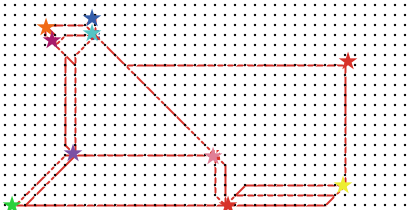
\includegraphics[width=0.5\columnwidth,height=6cm]{figures/networkDense}
          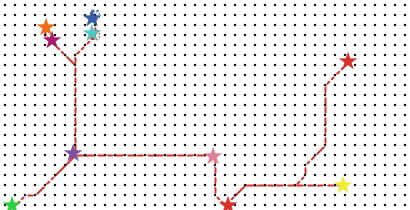
\includegraphics[width=0.5\columnwidth,height=6cm]{figures/networkLessDense}\\
          \bigskip
          \begin{justify}
          \textit{Sensibilité de la topologie du réseau au coefficient de renforcement $\gamma$. Gauche : $\gamma \sim 1$, réseau robuste. Droite : $\gamma >> 1$, réseau arborescent.}
          \end{justify}
          \end{column}
          \end{columns}
        \end{block}
        
        
      \end{column}
      
      
      \begin{column}{.49\textwidth}
      
        \begin{block}{Application : Corridor Optimal}
          \begin{columns}[t]
        \begin{column}{.95\textwidth}
        \begin{justify}
        \vspace{-2cm}
          Application abstraite : \textit{étant donné une distribution de noeuds à desservir (puits), quel est le corridor optimal pour une infrastructure à plus grande échelle (ex. : réseau ferré) pour laquelle les stations sont considérées comme des sources, au sens de l'optimalité multi-critères du réseau local auto-généré dans ce contexte ?}
          
          \bigskip
          $\rightarrow$ Exploration heuristique d'un espace arborescent d'implantations possibles ; obtention des fronts de Pareto pour les différents indicateurs ; choix de solutions optimales au sens de Pareto
          \vspace{1cm}
          \begin{columns}[t]
        \begin{column}{.48\textwidth}
          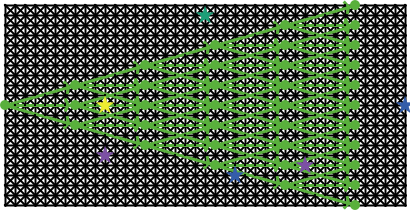
\includegraphics[width=\columnwidth,height=7cm]{figures/implantationtree}
          
          \textit{Arbre heuristique d'exploration des implantations.}
          \end{column}
          \begin{column}{.48\textwidth}
          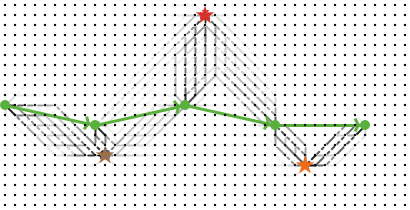
\includegraphics[width=\columnwidth,height=7cm]{figures/ImplantationTreeview}
          
          \textit{Exemple de réseau en cours de génération pour une implantation donnée.}
          \end{column}
          
          \end{columns}
          \vspace{1.5cm}
          
          \centering
          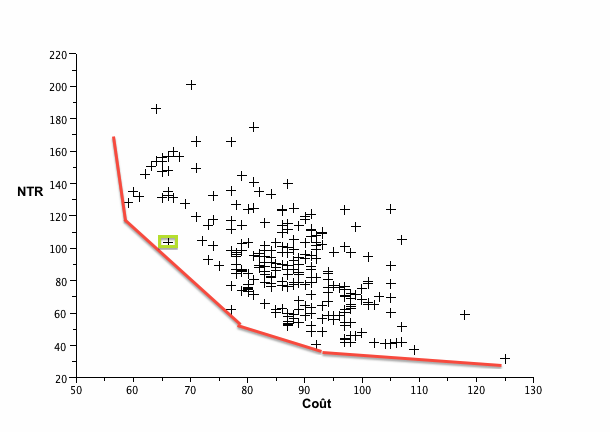
\includegraphics[width=0.33\columnwidth,height=9cm]{figures/implantationcntr}
          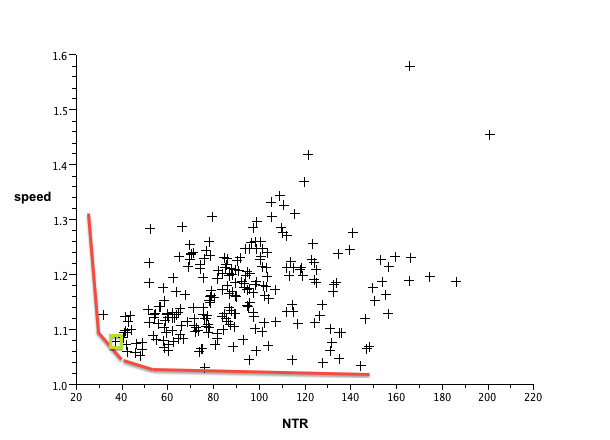
\includegraphics[width=0.33\columnwidth,height=9cm]{figures/implantationntrspeed}
          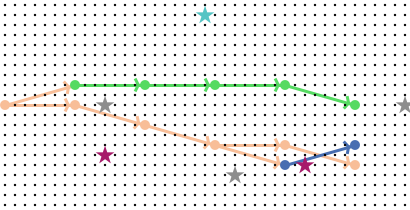
\includegraphics[width=0.33\columnwidth,height=9cm]{figures/paretosimplantation}
          
          \textit{Optimisation de Pareto : projection des configurations explorées dans l'espace des indicateurs, obtention du front de pareto ; configurations correspondant à trois points optimaux.}
         
          
          \end{justify}
          \end{column}
          \end{columns}
        \end{block}

        \begin{block}{Application : Desserte Optimale}
        \vspace{-1.5cm}
          \begin{columns}[t]
        \begin{column}{.95\textwidth}
        \begin{itemize}
          \item \begin{justify}Mission de prospective pour la mairie de Romainville : itinéraire d'une navette intra-urbaine avec points de desserte imposés.\end{justify}
          \bigskip
          \item \begin{justify} Problème type voyageur de commerce, mais multi-objectif (coût, vitesse, robustesse) : la génération de réseau \emph{bottom-up} par application du modèle sur un réseau initial construit par données géographiques réelles (réseau de rues) donne une solution proche du front de Pareto.\end{justify}
          \end{itemize}
          \vspace{2cm}
          
          {
          \centering
          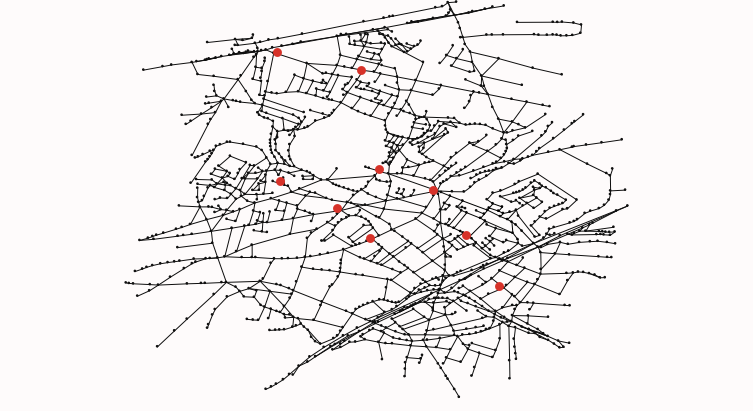
\includegraphics[width=0.32\columnwidth]{figures/tick1}
          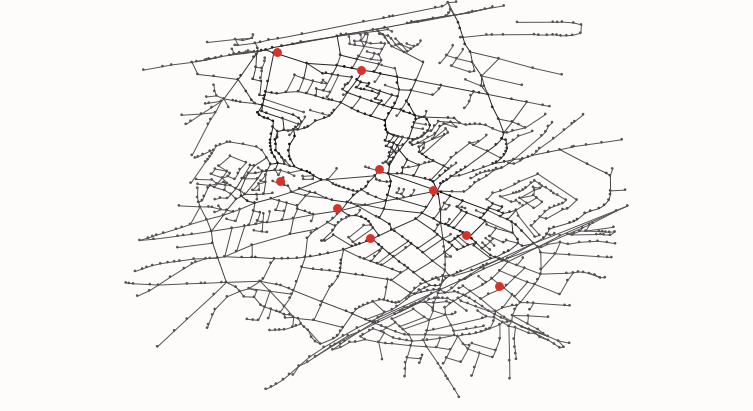
\includegraphics[width=0.32\columnwidth]{figures/tick10}
          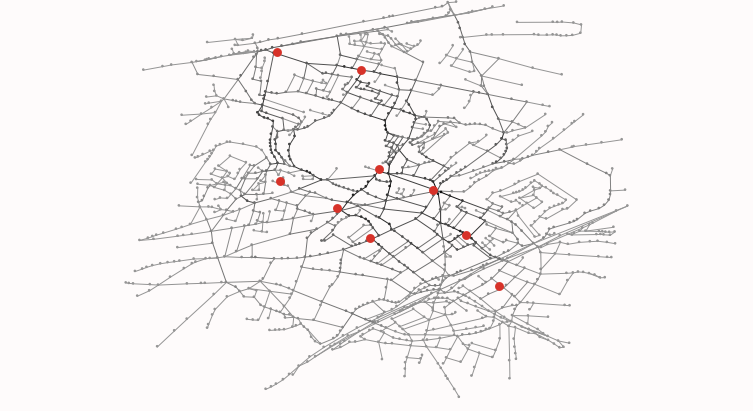
\includegraphics[width=0.32\columnwidth]{figures/tick20}\\
          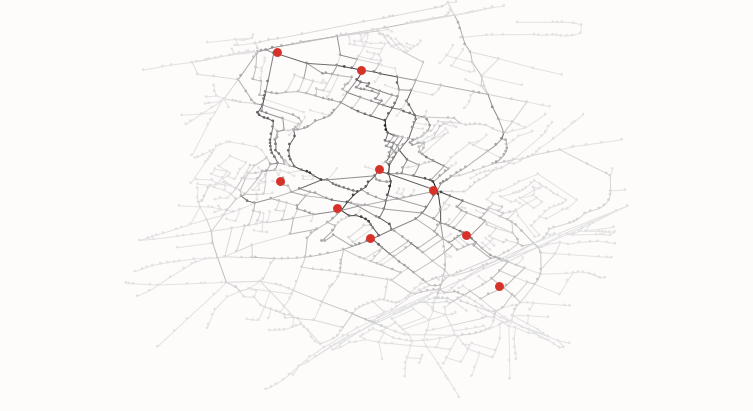
\includegraphics[width=0.32\columnwidth]{figures/tick50}
          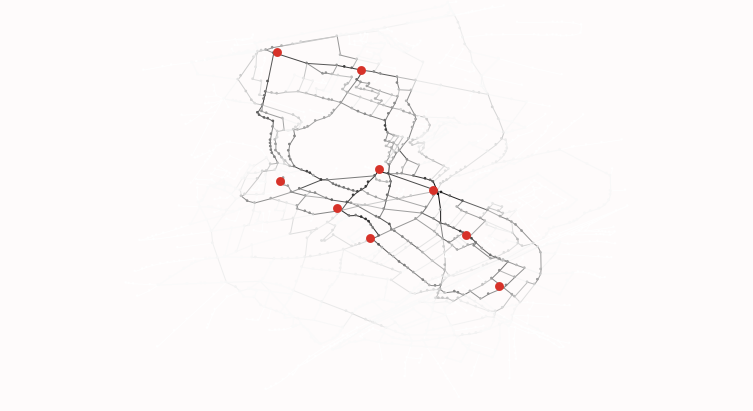
\includegraphics[width=0.32\columnwidth]{figures/tick101}
          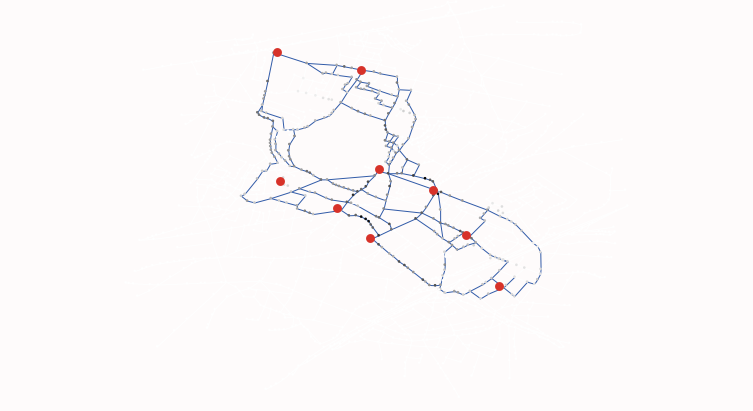
\includegraphics[width=0.32\columnwidth]{figures/reseauFinal}\\
          \bigskip
          \textit{Convergence progressive du réseau vers le réseau optimal desservant les points fixés (en rouge), en partant d'un réseau initial à diamètres égaux (réseau de rues).}\bigskip
          
          }
          \end{column}
          \end{columns}
        \end{block}

%        \begin{block}{Conclusion}
%         \begin{columns}[t]
%        \begin{column}{.95\textwidth}
%          
%          \end{column}
%          \end{columns}
%        \end{block}
        
        \begin{block}{References}
        {\tiny
        %\vspace{-1cm}
          \bibliographystyle{apalike}
          \bibliography{/Users/Juste/Documents/ComplexSystems/CityNetwork/Biblio/Bibtex/CityNetwork,biblio}
          }
        \end{block}
        
        
      \end{column}
    \end{columns}
  \end{frame}
\end{document}





